\documentclass[%
  crop,%
  tikz,%
  multi=false%
]{standalone}%
\usepackage[utf8]{luainputenc}%
\usepackage[no-math]{fontspec}%
\defaultfontfeatures{%
  Numbers={OldStyle,Proportional},%
  Ligatures=TeX,%
  Extension=.ttf,%
}%
\setmainfont[%
  UprightFont=*-Regular,%
  ItalicFont=*-Italic,%
  BoldFont=*-Bold,%
  BoldItalicFont=*-BoldItalic,%
]{Raleway}%
\setsansfont[%
  UprightFont=*-Regular,%
  ItalicFont=*-Italic,%
  BoldFont=*-Bold,%
  BoldItalicFont=*-BoldItalic,%
]{Raleway}%
\usepackage[frenchmath]{mathastext}%
\usepackage{amsmath}%
\usepackage{amssymb}%
\usepackage{mathrsfs}%
\usepackage{mathtools}%
\usepackage{siunitx}%
\usepackage[siunitx]{circuitikz}%
\usetikzlibrary{calc,backgrounds,arrows.meta,patterns,positioning}%
\ctikzset{bipoles/length=1.2cm}%

% Colors
\usepackage{xcolor}%
\definecolor{RoseauGreen}{HTML}{cad40e}%
\definecolor{RoseauGrey}{HTML}{adb9cb}%
\definecolor{RoseauBlue}{HTML}{234e83}%

\DeclareMathOperator{\sign}{sign}%

% Sets
\let\C\relax
\newcommand{\R}{\ensuremath{\mathbb{R}}} % Real
\newcommand{\N}{\ensuremath{\mathbb{N}}} % Natural
% \newcommand{\C}{\ensuremath{\mathbb{C}}} % Complexes
\newcommand{\B}{\ensuremath{\mathscr{B}}} % Electrical buses
\newcommand{\Ch}{\ensuremath{\mathscr{C}}} % Loads
\renewcommand{\L}{\ensuremath{\mathscr{L}}} % Lines
\renewcommand{\P}{\ensuremath{\mathscr{P}}} % Phases

% Phases
\newcommand{\arm}{\ensuremath{\mathrm{a}}}%
\newcommand{\brm}{\ensuremath{\mathrm{b}}}%
\newcommand{\crm}{\ensuremath{\mathrm{c}}}%
\newcommand{\nrm}{\ensuremath{\mathrm{n}}}%
\newcommand{\grm}{\ensuremath{\mathrm{g}}}%
\newcommand{\abrm}{\ensuremath{\mathrm{ab}}}%
\newcommand{\bcrm}{\ensuremath{\mathrm{bc}}}%
\newcommand{\carm}{\ensuremath{\mathrm{ca}}}%
\newcommand{\anrm}{\ensuremath{\mathrm{an}}}%
\newcommand{\bnrm}{\ensuremath{\mathrm{bn}}}%
\newcommand{\cnrm}{\ensuremath{\mathrm{cn}}}%
\newcommand{\agrm}{\ensuremath{\mathrm{ag}}}%
\newcommand{\bgrm}{\ensuremath{\mathrm{bg}}}%
\newcommand{\cgrm}{\ensuremath{\mathrm{cg}}}%
\newcommand{\ngrm}{\ensuremath{\mathrm{ng}}}%
\newcommand{\abcrm}{\ensuremath{\mathrm{abc}}}%
\newcommand{\abcnrm}{\ensuremath{\mathrm{abcn}}}%

% Transformer
\newcommand{\Xrm}{\ensuremath{\mathrm{X}}}%
\newcommand{\Yrm}{\ensuremath{\mathrm{Y}}}%
\newcommand{\Zrm}{\ensuremath{\mathrm{Z}}}%
\newcommand{\xrm}{\ensuremath{\mathrm{x}}}%
\newcommand{\yrm}{\ensuremath{\mathrm{y}}}%
\newcommand{\zrm}{\ensuremath{\mathrm{z}}}%
\newcommand{\Arm}{\ensuremath{\mathrm{A}}}%
\newcommand{\Brm}{\ensuremath{\mathrm{B}}}%
\newcommand{\Crm}{\ensuremath{\mathrm{C}}}%
\newcommand{\Nrm}{\ensuremath{\mathrm{N}}}%

% Indices or exponents
\newcommand{\cons}{\ensuremath{\mathrm{cons.}}}%
\renewcommand{\prod}{\ensuremath{\mathrm{prod.}}}%
\newcommand{\theo}{\ensuremath{\mathrm{th.}}}%
\newcommand{\const}{\ensuremath{\mathrm{const.}}}%

% Variables
\newcommand{\umax}{\ensuremath{U^{\max}}}%
\newcommand{\umaxnorm}{\ensuremath{U^{\max\,\text{norm.}}}}%
\newcommand{\umin}{\ensuremath{U^{\min}}}%
\newcommand{\uminnorm}{\ensuremath{U^{\min\,\text{norm.}}}}%
\newcommand{\unom}{\ensuremath{U^{\text{nom.}}}}%
\newcommand{\unomnorm}{\ensuremath{U^{\text{nom.}\,\text{norm.}}}}%
\newcommand{\uup}{\ensuremath{U^{\text{up}}}}%
\newcommand{\uupnorm}{\ensuremath{U^{\text{up}\,\text{norm.}}}}%
\newcommand{\uupprime}{\ensuremath{U^{\text{up}\,\prime}}}%
\newcommand{\udown}{\ensuremath{U^{\text{down}}}}%
\newcommand{\udownnorm}{\ensuremath{U^{\text{down}\,\text{norm.}}}}%
\newcommand{\udownprime}{\ensuremath{U^{\text{down}\,\prime}}}%
\newcommand{\smax}{\ensuremath{S^{\max}}}%
\newcommand{\pmax}{\ensuremath{P^{\max}}}%
\newcommand{\sproj}{\ensuremath{\underline{S^{\text{proj.}}}}}%
%

\begin{document}
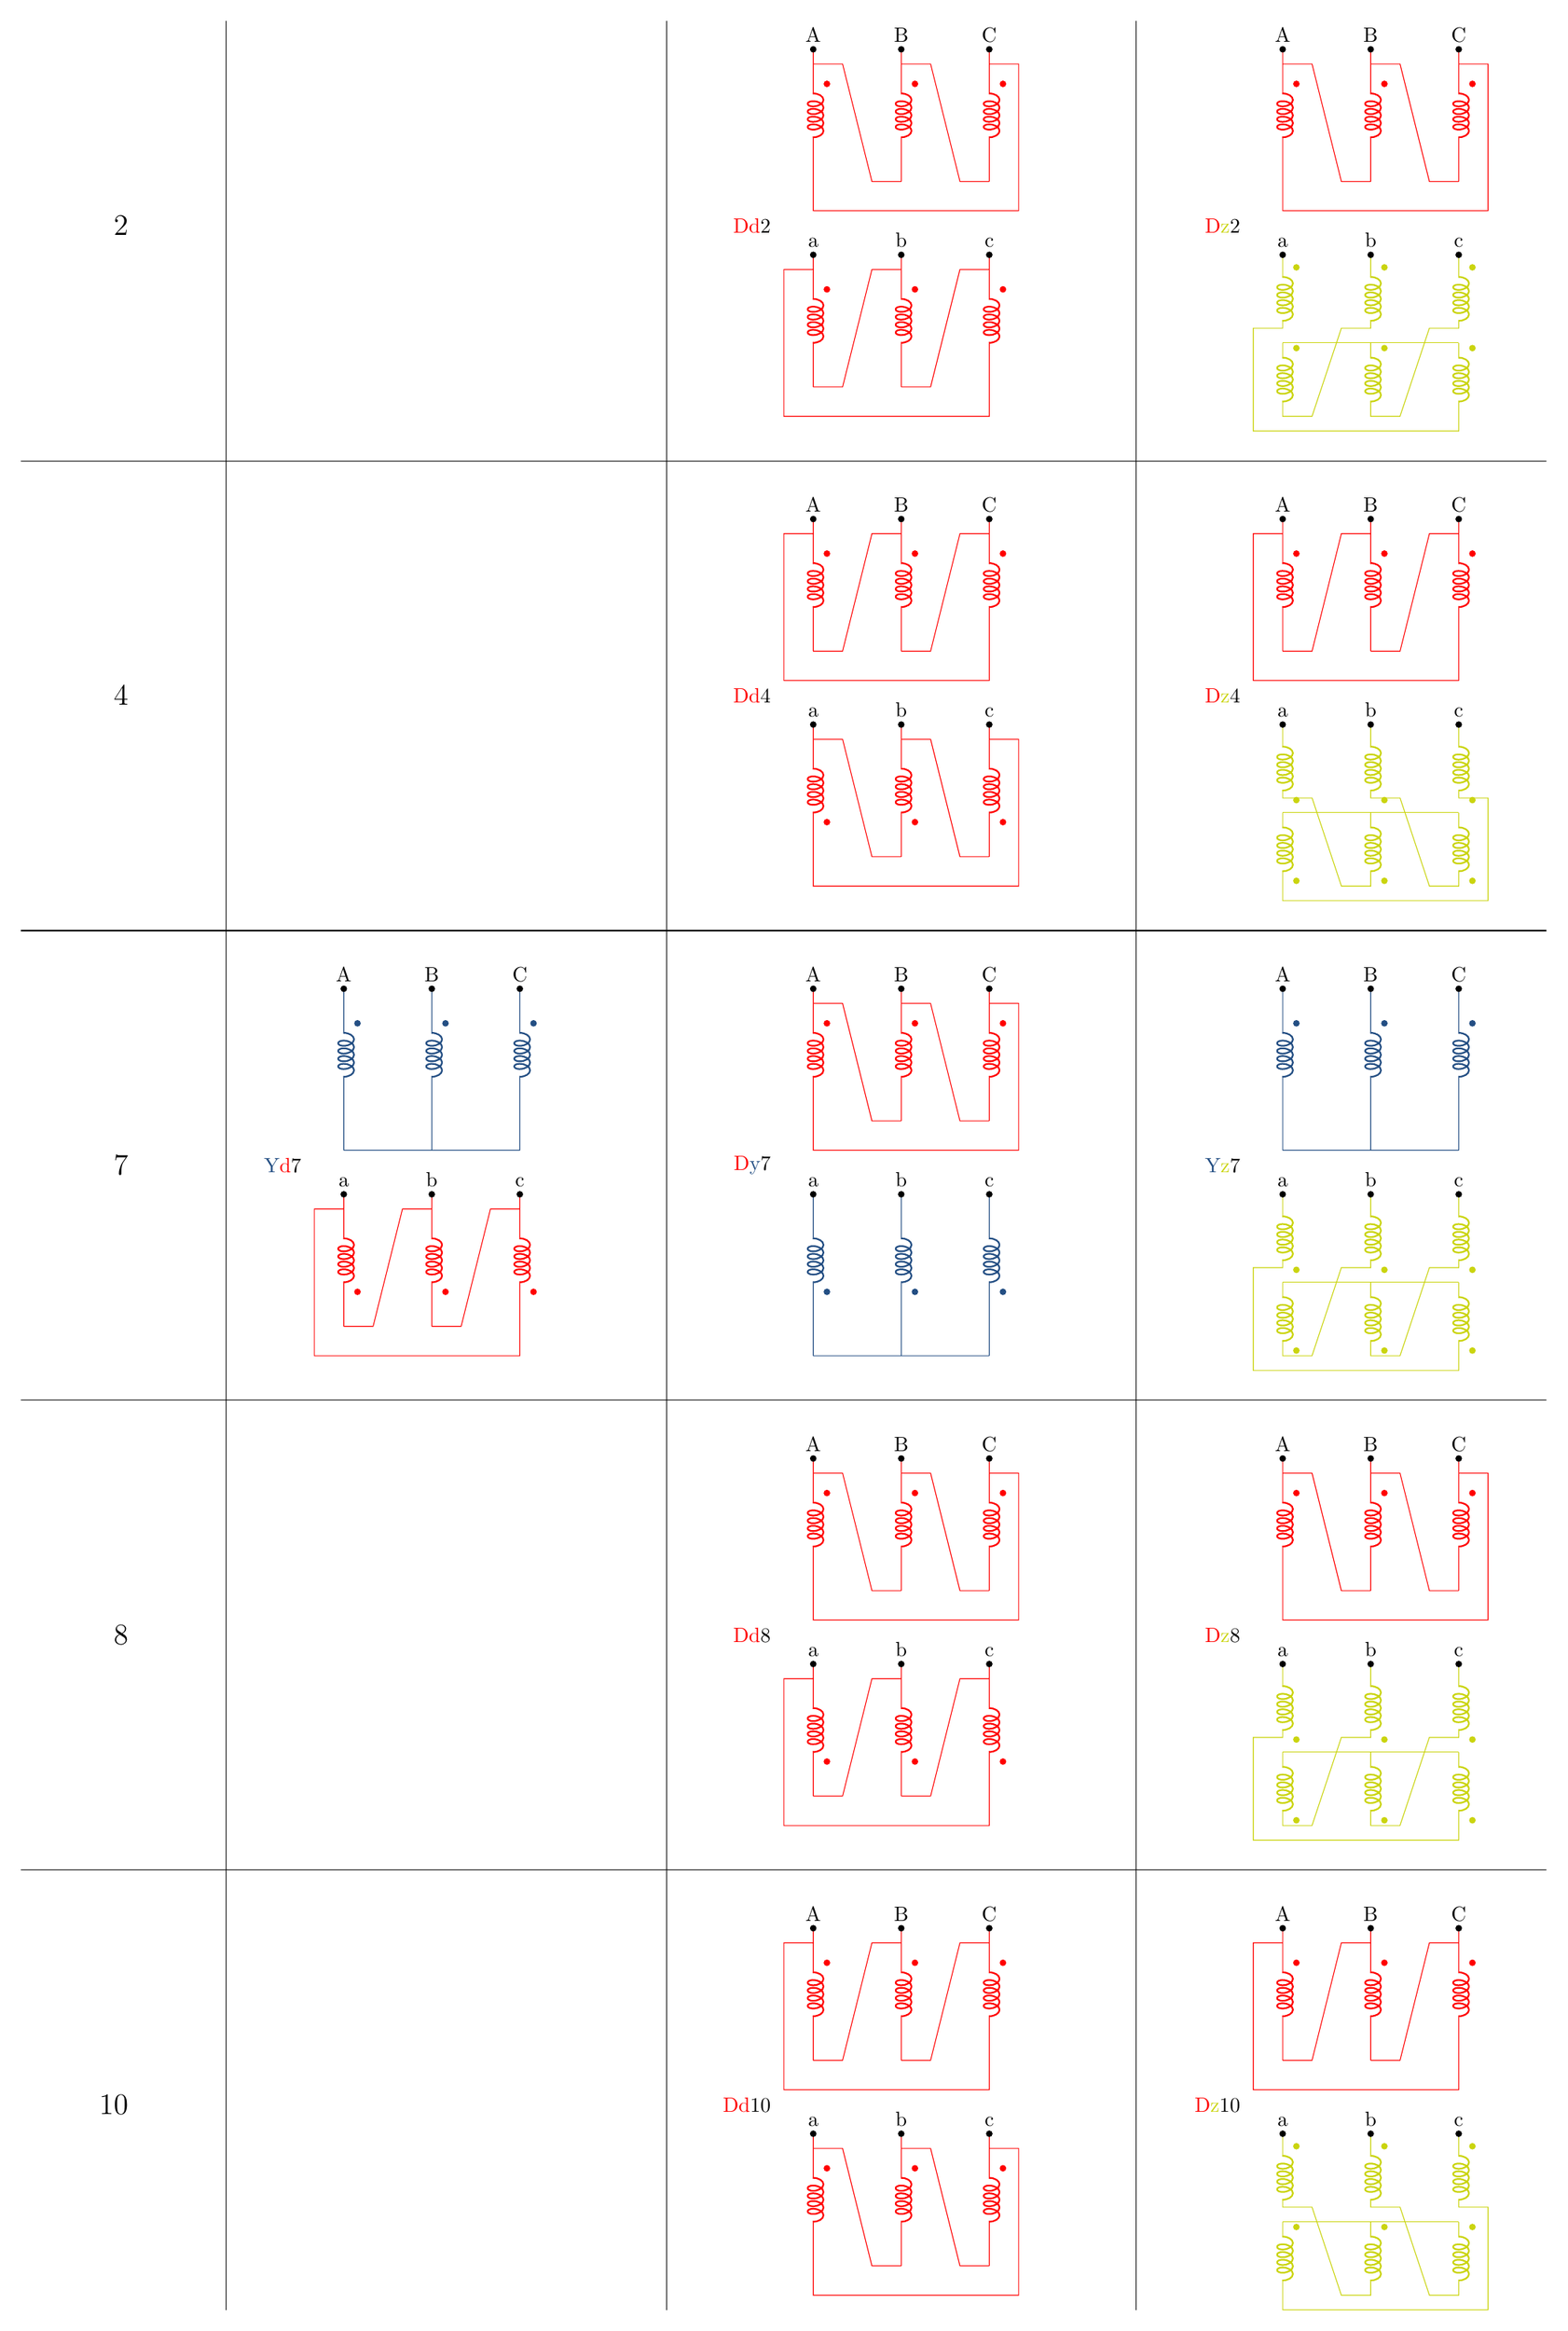
\begin{tikzpicture}[%
    show background rectangle,%
    tight background,%
    background rectangle/.style={fill=white}%
  ]
  %
% Definitions of windings
%
\pgfmathsetmacro{\yt}{0.25}%
\pgfmathsetmacro{\yzero}{0}%
\pgfmathsetmacro{\yone}{-0.5}%
\pgfmathsetmacro{\ytwo}{-1}%
\pgfmathsetmacro{\ythree}{-1.25}%
\pgfmathsetmacro{\yfour}{-2}%
\pgfmathsetmacro{\yfive}{-2.5}%
\pgfmathsetmacro{\ysix}{-2.75}%

\pgfmathsetmacro{\xAl}{0.0}%
\pgfmathsetmacro{\xA}{0.5}%
\pgfmathsetmacro{\xAr}{1.0}%
\pgfmathsetmacro{\xBl}{1.5}%
\pgfmathsetmacro{\xB}{2.0}%
\pgfmathsetmacro{\xBr}{2.5}%
\pgfmathsetmacro{\xCl}{3.0}%
\pgfmathsetmacro{\xC}{3.5}%
\pgfmathsetmacro{\xCr}{4.0}%

\ctikzset{european, straight voltages, bipoles/length=1.2cm, cute inductors}%

\tikzset{
  D direct/.pic={
    \draw[red,text=black]
    (\xA,\yt) node[circ,black]{} node[above]{A} to[L, -, name=X] (\xA,\yfour)%
    (\xB,\yt) node[circ,black]{} node[above]{B} to[L, -, name=Y] (\xB,\yfour)%
    (\xC,\yt) node[circ,black]{} node[above]{C} to[L, -, name=Z] (\xC,\yfour)%
    (\xA,\yfour) to[short, -] (\xAr,\yfour) to[short, -] (\xBl,\yzero) to[short, -] (\xB,\yzero)%
    (\xB,\yfour) to[short, -] (\xBr,\yfour) to[short, -] (\xCl,\yzero) to[short, -] (\xC,\yzero)%
    (\xC,\yfour) to[short, -] (\xC,\yfive) to[short, -] (\xAl,\yfive) to[short, -] (\xAl,\yzero) to[short, -] (\xA,\yzero);%
    \path[fill=red,draw=red]
    (X.ul dot) node[circ]{}%
    (Y.ul dot) node[circ]{}%
    (Z.ul dot) node[circ]{};%
    \path (\xAl,\yt) to (\xCr,\yt) to (\xCr,\ysix) to (\xAl,\ysix);% invisible path to center the pic
  },
  D inverse/.pic={
    \draw[red,text=black]
    (\xA,\yt) node[circ,black]{} node[above]{A} to[L, -, name=X] (\xA,\yfour)%
    (\xB,\yt) node[circ,black]{} node[above]{B} to[L, -, name=Y] (\xB,\yfour)%
    (\xC,\yt) node[circ,black]{} node[above]{C} to[L, -, name=Z] (\xC,\yfour)%
    (\xA,\yzero) to[short, -] (\xAr,\yzero) to[short, -] (\xBl,\yfour) to[short, -] (\xB,\yfour)%
    (\xB,\yzero) to[short, -] (\xBr,\yzero) to[short, -] (\xCl,\yfour) to[short, -] (\xC,\yfour)%
    (\xC,\yzero) to[short, -] (\xCr,\yzero) to[short, -] (\xCr,\yfive) to[short, -] (\xA,\yfive) to[short, -] (\xA,\yfour);%
    \path[fill=red,draw=red]
    (X.ul dot) node[circ]{}%
    (Y.ul dot) node[circ]{}%
    (Z.ul dot) node[circ]{};%
    \path (\xAl,\yt) to (\xCr,\yt) to (\xCr,\ysix) to (\xAl,\ysix);% invisible path to center the pic
  },
  d direct/.pic={
    \draw[red,text=black]
    (\xA,\yt) node[circ,black]{} node[above]{a} to[L, -, name=x] (\xA,\yfour)%
    (\xB,\yt) node[circ,black]{} node[above]{b} to[L, -, name=y] (\xB,\yfour)%
    (\xC,\yt) node[circ,black]{} node[above]{c} to[L, -, name=z] (\xC,\yfour)%
    (\xA,\yfour) to[short, -] (\xAr,\yfour) to[short, -] (\xBl,\yzero) to[short, -] (\xB,\yzero)%
    (\xB,\yfour) to[short, -] (\xBr,\yfour) to[short, -] (\xCl,\yzero) to[short, -] (\xC,\yzero)%
    (\xC,\yfour) to[short, -] (\xC,\yfive) to[short, -] (\xAl,\yfive) to[short, -] (\xAl,\yzero) to[short, -] (\xA,\yzero);%
    \path[fill=red,draw=red]
    (x.ul dot) node[circ]{}%
    (y.ul dot) node[circ]{}%
    (z.ul dot) node[circ]{};%
    \path (\xAl,\yt) to (\xCr,\yt) to (\xCr,\ysix) to (\xAl,\ysix);% invisible path to center the pic
  },
  d inverse/.pic={
    \draw[red,text=black]
    (\xA,\yt) node[circ,black]{} node[above]{a} to[L, -, name=x] (\xA,\yfour)%
    (\xB,\yt) node[circ,black]{} node[above]{b} to[L, -, name=y] (\xB,\yfour)%
    (\xC,\yt) node[circ,black]{} node[above]{c} to[L, -, name=z] (\xC,\yfour)%
    (\xA,\yzero) to[short, -] (\xAr,\yzero) to[short, -] (\xBl,\yfour) to[short, -] (\xB,\yfour)%
    (\xB,\yzero) to[short, -] (\xBr,\yzero) to[short, -] (\xCl,\yfour) to[short, -] (\xC,\yfour)%
    (\xC,\yzero) to[short, -] (\xCr,\yzero) to[short, -] (\xCr,\yfive) to[short, -] (\xA,\yfive) to[short, -] (\xA,\yfour);%
    \path[fill=red,draw=red]
    (x.ul dot) node[circ]{}%
    (y.ul dot) node[circ]{}%
    (z.ul dot) node[circ]{};%
    \path (\xAl,\yt) to (\xCr,\yt) to (\xCr,\ysix) to (\xAl,\ysix);% invisible path to center the pic
  },
  d direct reverse/.pic={
    \draw[red,text=black]
    (\xA,\yt) node[circ,black]{} node[above]{a} to[L, -, name=x] (\xA,\yfour)%
    (\xB,\yt) node[circ,black]{} node[above]{b} to[L, -, name=y] (\xB,\yfour)%
    (\xC,\yt) node[circ,black]{} node[above]{c} to[L, -, name=z] (\xC,\yfour)%
    (\xA,\yfour) to[short, -] (\xAr,\yfour) to[short, -] (\xBl,\yzero) to[short, -] (\xB,\yzero)%
    (\xB,\yfour) to[short, -] (\xBr,\yfour) to[short, -] (\xCl,\yzero) to[short, -] (\xC,\yzero)%
    (\xC,\yfour) to[short, -] (\xC,\yfive) to[short, -] (\xAl,\yfive) to[short, -] (\xAl,\yzero) to[short, -] (\xA,\yzero);%
    \path[fill=red,draw=red]
    (x.ur dot) node[circ]{}%
    (y.ur dot) node[circ]{}%
    (z.ur dot) node[circ]{};%
    \path (\xAl,\yt) to (\xCr,\yt) to (\xCr,\ysix) to (\xAl,\ysix);% invisible path to center the pic
  },
  d inverse reverse/.pic={
    \draw[red,text=black]
    (\xA,\yt) node[circ,black]{} node[above]{a} to[L, -, name=x] (\xA,\yfour)%
    (\xB,\yt) node[circ,black]{} node[above]{b} to[L, -, name=y] (\xB,\yfour)%
    (\xC,\yt) node[circ,black]{} node[above]{c} to[L, -, name=z] (\xC,\yfour)%
    (\xA,\yzero) to[short, -] (\xAr,\yzero) to[short, -] (\xBl,\yfour) to[short, -] (\xB,\yfour)%
    (\xB,\yzero) to[short, -] (\xBr,\yzero) to[short, -] (\xCl,\yfour) to[short, -] (\xC,\yfour)%
    (\xC,\yzero) to[short, -] (\xCr,\yzero) to[short, -] (\xCr,\yfive) to[short, -] (\xA,\yfive) to[short, -] (\xA,\yfour);%
    \path[fill=red,draw=red]
    (x.ur dot) node[circ]{}%
    (y.ur dot) node[circ]{}%
    (z.ur dot) node[circ]{};%
    \path (\xAl,\yt) to (\xCr,\yt) to (\xCr,\ysix) to (\xAl,\ysix);% invisible path to center the pic
  },
  Y/.pic={
    \draw[RoseauBlue, text=black]
    (\xA,\yt) node[circ,black]{} node[above]{A} to[L, -, name=X] (\xA,\yfour) to[short, -] (\xA,\yfive) %
    (\xB,\yt) node[circ,black]{} node[above]{B} to[L, -, name=Y] (\xB,\yfour) to[short, -] (\xB,\yfive) %
    (\xC,\yt) node[circ,black]{} node[above]{C} to[L, -, name=Z] (\xC,\yfour) to[short, -] (\xC,\yfive) %
    (\xA,\yfive) to[short, -] (\xC,\yfive);%
    \path[fill=RoseauBlue,draw=RoseauBlue]
    (X.ul dot) node[circ]{}%
    (Y.ul dot) node[circ]{}%
    (Z.ul dot) node[circ]{};%
    \path (\xAl,\yt) to (\xCr,\yt) to (\xCr,\ysix) to (\xAl,\ysix);% invisible path to center the pic
  },
  y/.pic={
    \draw[RoseauBlue, text=black]
    (\xA,\yt) node[circ,black]{} node[above]{a} to[L, -, name=x] (\xA,\yfour) to[short, -] (\xA,\yfive) %
    (\xB,\yt) node[circ,black]{} node[above]{b} to[L, -, name=y] (\xB,\yfour) to[short, -] (\xB,\yfive) %
    (\xC,\yt) node[circ,black]{} node[above]{c} to[L, -, name=z] (\xC,\yfour) to[short, -] (\xC,\yfive) %
    (\xA,\yfive) to[short, -] (\xC,\yfive);%
    \path[fill=RoseauBlue,draw=RoseauBlue]
    (x.ul dot) node[circ]{}%
    (y.ul dot) node[circ]{}%
    (z.ul dot) node[circ]{};%
    \path (\xAl,\yt) to (\xCr,\yt) to (\xCr,\ysix) to (\xAl,\ysix);% invisible path to center the pic
  },
  y reverse/.pic={
    \draw[RoseauBlue, text=black]
    (\xA,\yt) node[circ,black]{} node[above]{a} to[L, -, name=x] (\xA,\yfour) to[short, -] (\xA,\yfive) %
    (\xB,\yt) node[circ,black]{} node[above]{b} to[L, -, name=y] (\xB,\yfour) to[short, -] (\xB,\yfive) %
    (\xC,\yt) node[circ,black]{} node[above]{c} to[L, -, name=z] (\xC,\yfour) to[short, -] (\xC,\yfive) %
    (\xA,\yfive) to[short, -] (\xC,\yfive);%
    \path[fill=RoseauBlue,draw=RoseauBlue]
    (x.ur dot) node[circ]{}%
    (y.ur dot) node[circ]{}%
    (z.ur dot) node[circ]{};%
    \path (\xAl,\yt) to (\xCr,\yt) to (\xCr,\ysix) to (\xAl,\ysix);% invisible path to center the pic
  },
  z direct/.pic={
    \draw[RoseauGreen, text=black] (\xA,\yt) node[circ,black]{} node[above]{a}%
    to[short, -] (\xA, \yzero)%
    to[L, name=x1] (\xA,\ytwo)%
    to[short, -] (\xAl, \ytwo)%
    to[short, -] (\xAl, \ysix)%
    to[short, -] (\xC,\ysix)%
    to[short, -] (\xC,\yfive)%
    to[L, mirror, name=z2] (\xC,\ythree);%
    \draw[RoseauGreen, text=black] (\xB,\yt) node[circ,black]{} node[above]{b}%
    to[short, -] (\xB, \yzero)%
    to[L, name=y1] (\xB,\ytwo)%
    to[short, -] (\xBl,\ytwo)%
    to[short, -] (\xAr,\yfive)%
    to[short, -] (\xA,\yfive)%
    to[L, mirror, name=x2] (\xA,\ythree);%
    \draw[RoseauGreen, text=black] (\xC,\yt) node[circ,black]{} node[above]{c}%
    to[short, -] (\xC, \yzero)%
    to[L, name=z1] (\xC,\ytwo)%
    to[short, -] (\xCl,\ytwo)%
    to[short, -] (\xBr,\yfive)%
    to[short, -] (\xB,\yfive)%
    to[L, mirror, name=y2] (\xB,\ythree);%
    \draw[RoseauGreen, text=black] (\xA,\ythree) to[short, -] (\xC,\ythree);
    \path[fill=RoseauGreen,draw=RoseauGreen]
    (x1.ul dot) node[circ]{}%
    (x2.ur dot) node[circ]{}%
    (y1.ul dot) node[circ]{}%
    (y2.ur dot) node[circ]{}%
    (z1.ul dot) node[circ]{}%
    (z2.ur dot) node[circ]{};%
    \path (\xAl,\yt) to (\xCr,\yt) to (\xCr,\ysix) to (\xAl,\ysix);% invisible path to center the pic
  },
  z inverse/.pic={
    \draw[RoseauGreen, text=black] (\xA,\yt) node[circ,black]{} node[above]{a}%
    to[short, -] (\xA, \yzero)%
    to[L, name=x1] (\xA,\ytwo)%
    to[short, -] (\xAr, \ytwo)%
    to[short, -] (\xBl, \yfive)%
    to[short, -] (\xB,\yfive)%
    to[L, mirror, name=y2] (\xB,\ythree);%
    \draw[RoseauGreen, text=black] (\xB,\yt) node[circ,black]{} node[above]{b}%
    to[short, -] (\xB, \yzero)%
    to[L, name=y1] (\xB,\ytwo)%
    to[short, -] (\xBr,\ytwo)%
    to[short, -] (\xCl,\yfive)%
    to[short, -] (\xC,\yfive)%
    to[L, mirror, name=z2] (\xC,\ythree);%
    \draw[RoseauGreen, text=black] (\xC,\yt) node[circ,black]{} node[above]{c}%
    to[short, -] (\xC, \yzero)%
    to[L, name=z1] (\xC,\ytwo)%
    to[short, -] (\xCr,\ytwo)%
    to[short, -] (\xCr,\ysix)%
    to[short, -] (\xA,\ysix)%
    to[short, -] (\xA,\yfive)%
    to[L, mirror, name=x2] (\xA,\ythree);%
    \draw[RoseauGreen, text=black] (\xA,\ythree) to[short, -] (\xC,\ythree);
    \path[fill=RoseauGreen,draw=RoseauGreen]
    (x1.ul dot) node[circ]{}%
    (x2.ur dot) node[circ]{}%
    (y1.ul dot) node[circ]{}%
    (y2.ur dot) node[circ]{}%
    (z1.ul dot) node[circ]{}%
    (z2.ur dot) node[circ]{};%
    \path (\xAl,\yt) to (\xCr,\yt) to (\xCr,\ysix) to (\xAl,\ysix);% invisible path to center the pic
  },
  z direct reverse/.pic={
    \draw[RoseauGreen, text=black] (\xA,\yt) node[circ,black]{} node[above]{a}%
    to[short, -] (\xA, \yzero)%
    to[L, name=x1] (\xA,\ytwo)%
    to[short, -] (\xAl, \ytwo)%
    to[short, -] (\xAl, \ysix)%
    to[short, -] (\xC,\ysix)%
    to[short, -] (\xC,\yfive)%
    to[L, mirror, name=z2] (\xC,\ythree);%
    \draw[RoseauGreen, text=black] (\xB,\yt) node[circ,black]{} node[above]{b}%
    to[short, -] (\xB, \yzero)%
    to[L, name=y1] (\xB,\ytwo)%
    to[short, -] (\xBl,\ytwo)%
    to[short, -] (\xAr,\yfive)%
    to[short, -] (\xA,\yfive)%
    to[L, mirror, name=x2] (\xA,\ythree);%
    \draw[RoseauGreen, text=black] (\xC,\yt) node[circ,black]{} node[above]{c}%
    to[short, -] (\xC, \yzero)%
    to[L, name=z1] (\xC,\ytwo)%
    to[short, -] (\xCl,\ytwo)%
    to[short, -] (\xBr,\yfive)%
    to[short, -] (\xB,\yfive)%
    to[L, mirror, name=y2] (\xB,\ythree);%
    \draw[RoseauGreen, text=black] (\xA,\ythree) to[short, -] (\xC,\ythree);
    \path[fill=RoseauGreen,draw=RoseauGreen]
    (x1.ur dot) node[circ]{}%
    (x2.ul dot) node[circ]{}%
    (y1.ur dot) node[circ]{}%
    (y2.ul dot) node[circ]{}%
    (z1.ur dot) node[circ]{}%
    (z2.ul dot) node[circ]{};%
    \path (\xAl,\yt) to (\xCr,\yt) to (\xCr,\ysix) to (\xAl,\ysix);% invisible path to center the pic
  },
  z inverse reverse/.pic={
    \draw[RoseauGreen, text=black] (\xA,\yt) node[circ,black]{} node[above]{a}%
    to[short, -] (\xA, \yzero)%
    to[L, name=x1] (\xA,\ytwo)%
    to[short, -] (\xAr, \ytwo)%
    to[short, -] (\xBl, \yfive)%
    to[short, -] (\xB,\yfive)%
    to[L, mirror, name=y2] (\xB,\ythree);%
    \draw[RoseauGreen, text=black] (\xB,\yt) node[circ,black]{} node[above]{b}%
    to[short, -] (\xB, \yzero)%
    to[L, name=y1] (\xB,\ytwo)%
    to[short, -] (\xBr,\ytwo)%
    to[short, -] (\xCl,\yfive)%
    to[short, -] (\xC,\yfive)%
    to[L, mirror, name=z2] (\xC,\ythree);%
    \draw[RoseauGreen, text=black] (\xC,\yt) node[circ,black]{} node[above]{c}%
    to[short, -] (\xC, \yzero)%
    to[L, name=z1] (\xC,\ytwo)%
    to[short, -] (\xCr,\ytwo)%
    to[short, -] (\xCr,\ysix)%
    to[short, -] (\xA,\ysix)%
    to[short, -] (\xA,\yfive)%
    to[L, mirror, name=x2] (\xA,\ythree);%
    \draw[RoseauGreen, text=black] (\xA,\ythree) to[short, -] (\xC,\ythree);
    \path[fill=RoseauGreen,draw=RoseauGreen]
    (x1.ur dot) node[circ]{}%
    (x2.ul dot) node[circ]{}%
    (y1.ur dot) node[circ]{}%
    (y2.ul dot) node[circ]{}%
    (z1.ur dot) node[circ]{}%
    (z2.ul dot) node[circ]{};%
    \path (\xAl,\yt) to (\xCr,\yt) to (\xCr,\ysix) to (\xAl,\ysix);% invisible path to center the pic
  },
  empty/.pic={
    % empty pic to align the other pics
    \path (\xA,\yt) node[above]{\phantom{A}} (\xB,\yt) node[above]{\phantom{B}} (\xC,\yt) node[above]{\phantom{C}};%
    \path (\xAl,\yt) to (\xCr,\yt) to (\xCr,\ysix) to (\xAl,\ysix);% invisible path to center the pic
  },
  clock/.pic={
    \path (\xB,\yt) node[above]{\phantom{B}};%
    \path (\xAr,\yt) to (\xCl,\yt) to (\xCl,\ysix) to (\xAr,\ysix);% invisible path to center the pic
  },
}
%

  % Phase displacement = 2
  \begin{scope}[local bounding box=C2, shift={(0,0)}]
    \pic at (0,0) {clock};%
    \pic at (0,-3.5) {clock};%
  \end{scope}
  \node[left=-2.0 of C2, node font=\Large] (C2 legend) {2};%
  \begin{scope}[local bounding box=Yy2, shift={(6,0)}]
    \pic at (0,0) {empty};%
    \pic at (0,-3.5) {empty};%
  \end{scope}
  \node[left=0.1 of Yy2] (Yy2 legend) {\phantom{Yy2}};%
  \begin{scope}[local bounding box=Dd2, shift={(14,0)}]
    \pic at (0,0) {D inverse};%
    \pic at (0,-3.5) {d direct};%
  \end{scope}
  \node[left=0.1 of Dd2] (Dd2 legend) {\textcolor{red}{Dd}2};%
  \begin{scope}[local bounding box=Dz2, shift={(22,0)}]
    \pic at (0,0) {D inverse};%
    \pic at (0,-3.5) {z direct};%
  \end{scope}
  \node[left=0.1 of Dz2] (Dz2 legend) {\textcolor{red}{D}\textcolor{RoseauGreen}{z}2};%

  % Phase displacement = 4
  \begin{scope}[local bounding box=C4, shift={(0,-8)}]
    \pic at (0,0) {clock};%
    \pic at (0,-3.5) {clock};%
  \end{scope}
  \node[left=-2.0 of C4, node font=\Large] (C4 legend) {4};%
  \begin{scope}[local bounding box=Yy4, shift={(6,-8)}]
    \pic at (0,0) {empty};%
    \pic at (0,-3.5) {empty};%
  \end{scope}
  \node[left=0.1 of Yy4] (Yy4 legend) {\phantom{Yy4}};%
  \begin{scope}[local bounding box=Dd4, shift={(14,-8)}]
    \pic at (0,0) {D direct};%
    \pic at (0,-3.5) {d inverse reverse};%
  \end{scope}
  \node[left=0.1 of Dd4] (Dd4 legend) {\textcolor{red}{Dd}4};%
  \begin{scope}[local bounding box=Dz4, shift={(22,-8)}]
    \pic at (0,0) {D direct};%
    \pic at (0,-3.5) {z inverse reverse};%
  \end{scope}
  \node[left=0.1 of Dz4] (Dz4 legend) {\textcolor{red}{D}\textcolor{RoseauGreen}{z}4};%

  % Phase displacement = 7
  \begin{scope}[local bounding box=C7, shift={(0,-16)}]
    \pic at (0,0) {clock};%
    \pic at (0,-3.5) {clock};%
  \end{scope}
  \node[left=-2.0 of C7, node font=\Large] (C7 legend) {7};%
  \begin{scope}[local bounding box=Yd7, shift={(6,-16)}]
    \pic at (0,0) {Y};%
    \pic at (0,-3.5) {d direct reverse};%
  \end{scope}
  \node[left=0.1 of Yd7] (Yd7 legend) {\textcolor{RoseauBlue}{Y}\textcolor{red}{d}7};%
  \begin{scope}[local bounding box=Dy7, shift={(14,-16)}]
    \pic at (0,0) {D inverse};%
    \pic at (0,-3.5) {y reverse};%
  \end{scope}
  \node[left=0.1 of Dy7] (Dy7 legend) {\textcolor{red}{D}\textcolor{RoseauBlue}{y}7};%
  \begin{scope}[local bounding box=Yz7, shift={(22,-16)}]
    \pic at (0,0) {Y};%
    \pic at (0,-3.5) {z direct reverse};%
  \end{scope}
  \node[left=0.1 of Yz7] (Yz7 legend) {\textcolor{RoseauBlue}{Y}\textcolor{RoseauGreen}{z}7};%

  % Phase displacement = 8
  \begin{scope}[local bounding box=C8, shift={(0,-24)}]
    \pic at (0,0) {clock};%
    \pic at (0,-3.5) {clock};%
  \end{scope}
  \node[left=-2.0 of C8, node font=\Large] (C8 legend) {8};%
  \begin{scope}[local bounding box=Yy8, shift={(6,-24)}]
    \pic at (0,0) {empty};%
    \pic at (0,-3.5) {empty};%
  \end{scope}
  \node[left=0.1 of Yy8] (Yy8 legend) {\phantom{Yy8}};%
  \begin{scope}[local bounding box=Dd8, shift={(14,-24)}]
    \pic at (0,0) {D inverse};%
    \pic at (0,-3.5) {d direct reverse};%
  \end{scope}
  \node[left=0.1 of Dd8] (Dd8 legend) {\textcolor{red}{Dd}8};%
  \begin{scope}[local bounding box=Dz8, shift={(22,-24)}]
    \pic at (0,0) {D inverse};%
    \pic at (0,-3.5) {z direct reverse};%
  \end{scope}
  \node[left=0.1 of Dz8] (Dz8 legend) {\textcolor{red}{D}\textcolor{RoseauGreen}{z}8};%

  % Phase displacement = 10
  \begin{scope}[local bounding box=C10, shift={(0,-32)}]
    \pic at (0,0) {clock};%
    \pic at (0,-3.5) {clock};%
  \end{scope}
  \node[left=-2.0 of C10, node font=\Large] (C10 legend) {10};%
  \begin{scope}[local bounding box=Yy10, shift={(6,-32)}]
    \pic at (0,0) {empty};%
    \pic at (0,-3.5) {empty};%
  \end{scope}
  \node[left=0.1 of Yy10] (Yy10 legend) {\phantom{Yy10}};%
  \begin{scope}[local bounding box=Dd10, shift={(14,-32)}]
    \pic at (0,0) {D direct};%
    \pic at (0,-3.5) {d inverse};%
  \end{scope}
  \node[left=0.1 of Dd10] (Dd10 legend) {\textcolor{red}{Dd}10};%
  \begin{scope}[local bounding box=Dz10, shift={(22,-32)}]
    \pic at (0,0) {D direct};%
    \pic at (0,-3.5) {z inverse};%
  \end{scope}
  \node[left=0.1 of Dz10] (Dz10 legend) {\textcolor{red}{D}\textcolor{RoseauGreen}{z}10};%

  % Add clock numbers coordinates to align the horizontal separators
  \coordinate[left=0.0 of C2] (C2l);%
  \coordinate[left=0.0 of C4] (C4l);%
  \coordinate[left=0.0 of C7] (C7l);%
  \coordinate[left=0.0 of C8] (C8l);%
  \coordinate[left=0.0 of C10] (C10l);%
  \coordinate[right=1.0 of Dz2] (C2r);%
  \coordinate[right=1.0 of Dz4] (C4r);%
  \coordinate[right=1.0 of Yz7] (C7r);%
  \coordinate[right=1.0 of Dz8] (C8r);%
  \coordinate[right=1.0 of Dz10] (C10r);%

  % Draw horizontal separators
  \draw ($(C2l.south west)!0.5!(C4l.north west)$) -- ($(C2r.south east)!0.5!(C4r.north east)$);%
  \draw ($(C4l.south west)!0.5!(C7l.north west)$) -- ($(C4r.south east)!0.5!(C7r.north east)$);%
  \draw ($(C7l.south west)!0.5!(C8l.north west)$) -- ($(C7r.south east)!0.5!(C8r.north east)$);%
  \draw ($(C8l.south west)!0.5!(C10l.north west)$) -- ($(C8r.south east)!0.5!(C10r.north east)$);%

  % Draw vertical separators
  \draw ($(C2.north east)!0.5!(Yy2.north west)$) -- ($(C10.south east)!0.5!(Yy10.south west)$);%
  \draw ($(Yy2.north east)!0.5!(Dd2.north west)$) -- ($(Yy10.south east)!0.5!(Dd10.south west)$);%
  \draw ($(Dd2.north east)!0.5!(Dz2.north west)$) -- ($(Dd10.south east)!0.5!(Dz10.south west)$);%
\end{tikzpicture}
\end{document}
% Local Variables:
% mode: latex
% TeX-engine: luatex
% TeX-source-correlate-method-active: synctex
% ispell-local-dictionary: "british"
% coding: utf-8
% LaTeX-indent-level: 2
% fill-column: 120
% End:
